Agents, a local broker, and a map service are deployed on-premises and can facilitate the computation of the path in this setup. Agents can communicate with each other to agree on who will initiate the computation. Figure \ref{fig:local_services} shows how local services are deployed. Local broker and map services need to be accessible for all agents to communicate and map selection and therefore in most cases those services would be deployed on a stand-alone server in the same subnet as agents.

\begin{figure}[H]
    \centering
    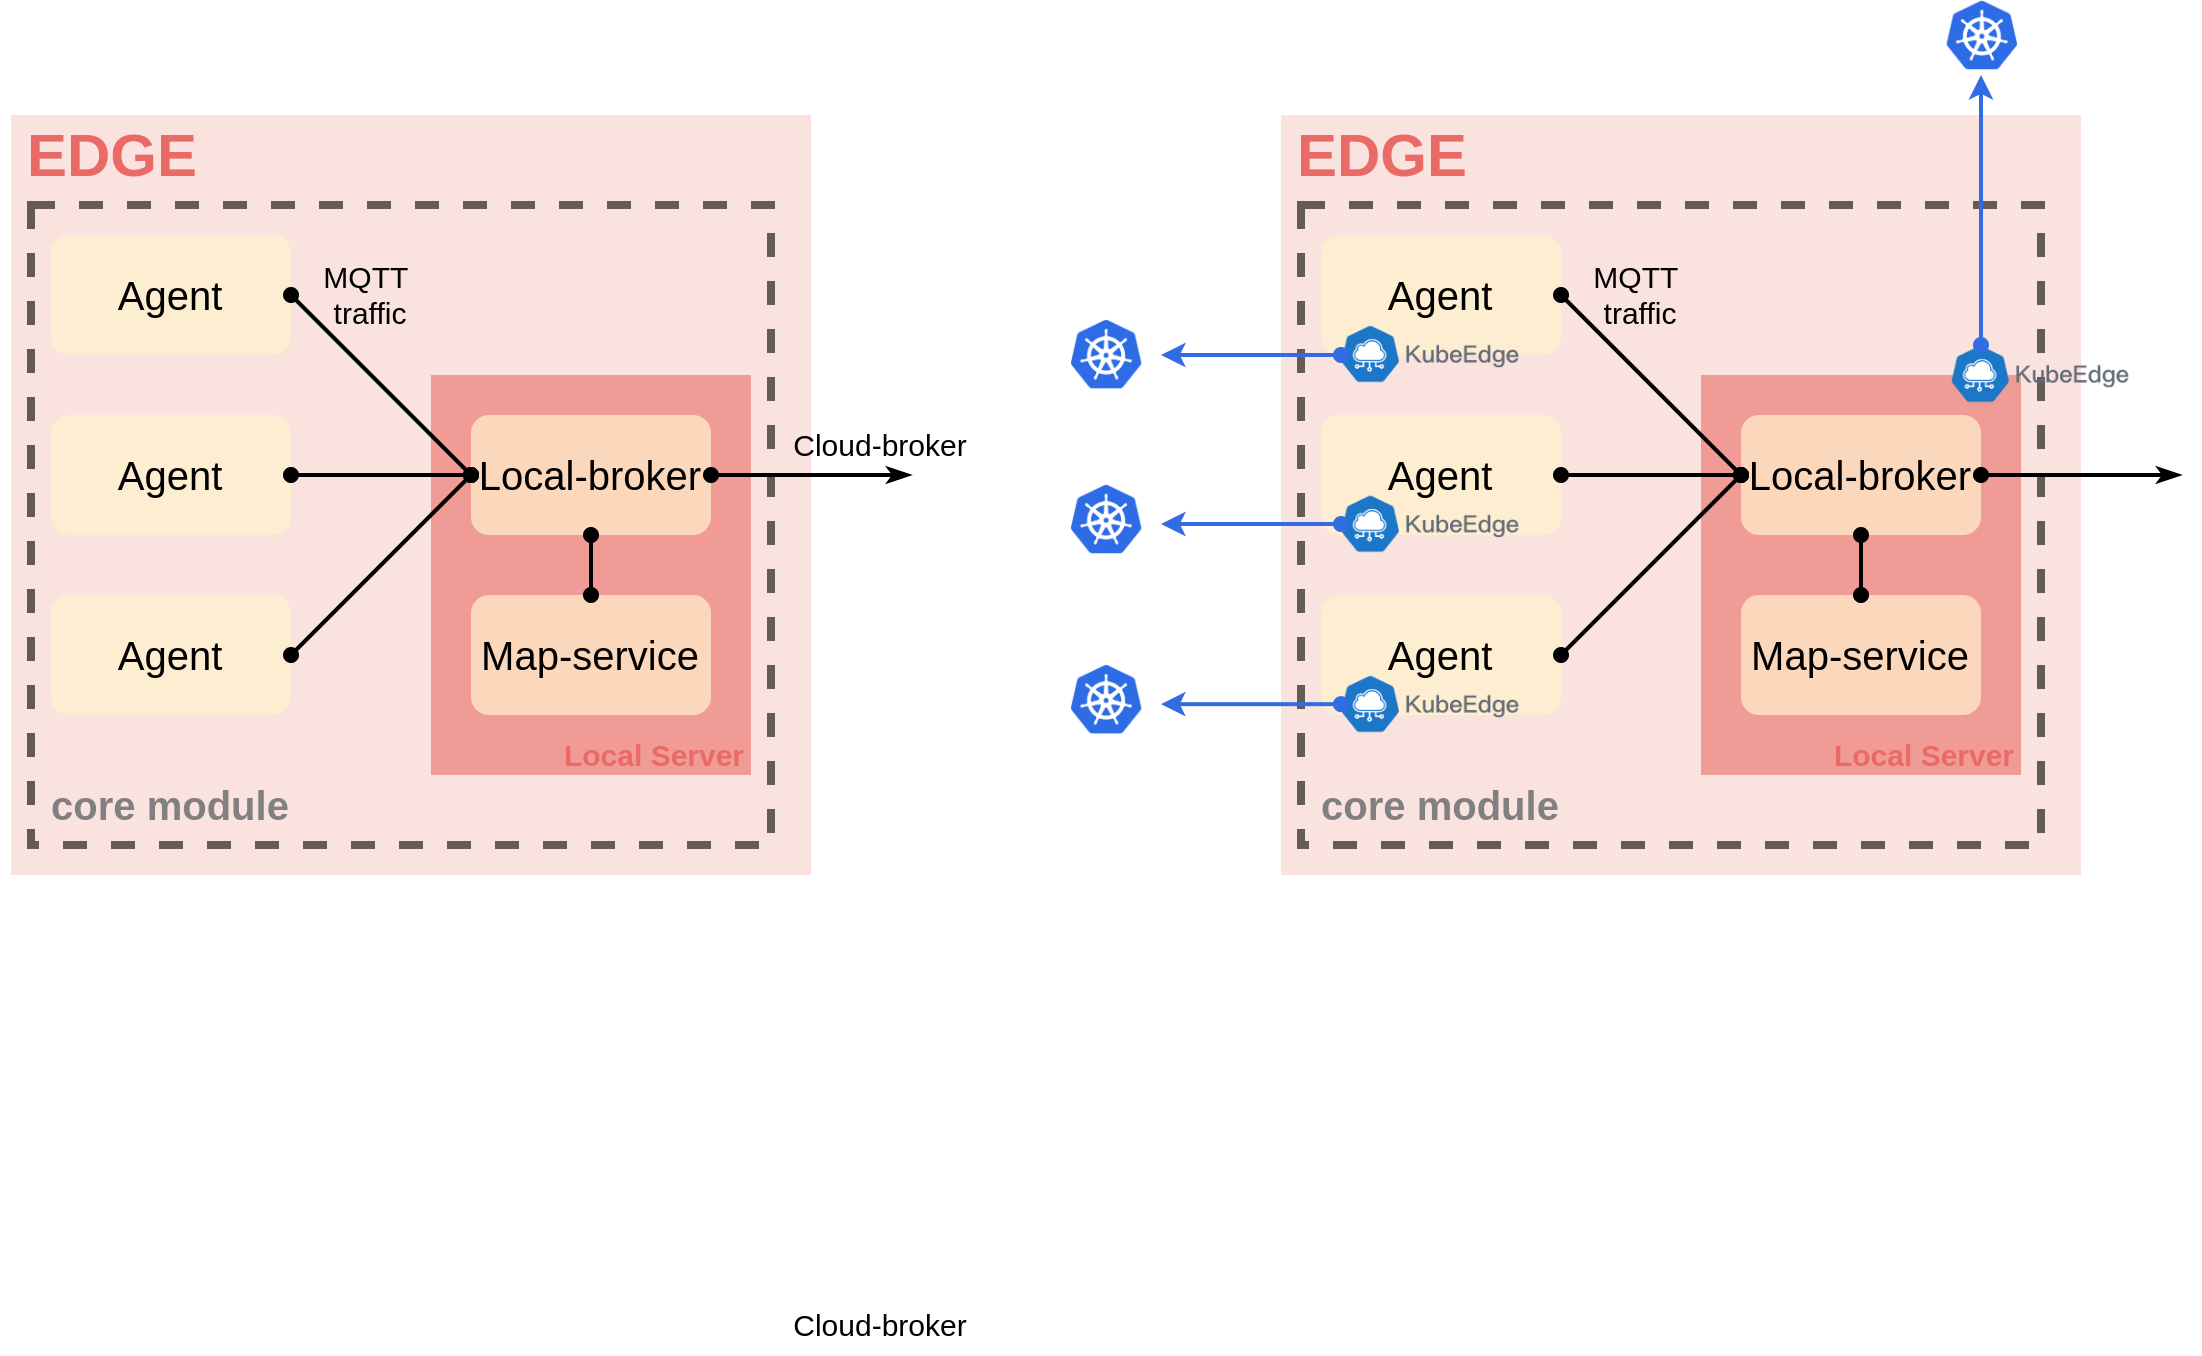
\includegraphics[width=0.5\textwidth]{pictures/local_service.png}
    \caption{ Local services system design }
    \label{fig:local_services}
\end{figure}

This design can be extended, by deploying an edge agent on the same server as a map service and a broker. It would allow performing path computation with help of an edge agent which would have a higher resource profile than agents.

Agents can be deployed in a different way, depending on implementation. Preferably it should be a single binary package that could be deployed on machines with low resource profiles. All the agents need to have an ID or NAME assigned to them, and those have to be unique in the scope of the system. They should also be given information about the IP/URL of the local broker and a way to authenticate themselves. 

Map service and broker are more flexible in case of deployment because those services would probably be deployed on a stand-alone server with a high resource profile. recommended way would be to use a containers orchestrator such as solutions like Kubernetes or docker swarm and deploy the as containers/pods. It would assure the reliability and maintainability of those services. Otherwise, those can also be deployed on bare metal or in virtual machines.